%
% sat.tex -- SAT
%
% (c) 2011 Prof Dr Andreas Mueller, Hochschule Rapperswil
%
\section{SAT}
\rhead{SAT}
\index{Cook, Steven}%
\index{Levin, Leonid}%
Bislang ist noch nicht klar, dass es überhaupt NP-vollständige
Problem gibt. Dies änderte sich mit dem Satz von Cook und Levin,
der beweist, dass \textsl{SAT} NP-vollständig ist.

\begin{satz}[Cook-Levin]
\label{cooklevin}
\textsl{SAT} ist NP-vollständig.
\end{satz}

\subsection{SUDOKU und SAT\label{subsection:sudoku-und-sat}}
\index{Sudoku}
Als Vorstufe der angestrebten Erkenntnis, dass sich jedes Problem auf \textsl{SAT}
reduzieren l"asst, wollen wir zeigen, dass sich die Frage nach der
L"osbarkeit eines Sudoku-R"atsels auf \textsl{SAT} reduzieren l"asst.

Ein $n$-Sudoku ist ein $n^2\times n^2$-Feld, welches mit $n^2$ verschiedenen
Zeichen aus einer Menge $\Sigma$ so gef"ullt werden muss,
dass in jeder Zeile, jeder Spalte
und in jedem der $n\times n$-Unterquadrate jedes Zeichen genau einmal
vorkommt.
Die aus R"atselspalten von Zeitungen bekannten $3$-Sudokus verwenden
die Ziffern $1$ bis $9$ f"ur $\Sigma$.
Einige der Zeichen sind bereits vorgegeben, die leeren Felder m"ussen
so gef"ullt werden, dass die Regeln nicht verletzt werden.
Abbildung~\ref{sudoku} zeigt ein l"osbares $3$-Sudoku-R"atsel.
\begin{figure}
\begin{center}
\includegraphics[width=0.4\hsize]{images/sudoku-1.pdf}
\end{center}
\caption{$3$-Sudoku, die hellen Ziffern zeigen, dass die Vorgabe (dunkle
Ziffern) erf"ullbar ist, das $3$-Sudoko ist l"osbar.\label{sudoku}}
\end{figure}
Wir schreiben
\begin{align*}
\textsl{SUDOKU}
=
\{\langle S\rangle\;|\; \text{$S$ ist ein l"osbares $n$-Sudoku}\}.
\end{align*}

Ob ein $n$-Sudoku l"osbar ist, ist sicher entscheidbar: man kann alle
$|\Sigma|^{n^2\cdot n^2}=n^{2n^4}$ m"oglichen Belegungen des Feldes mit
Zeichen durchprobieren, was aber nat"urlich exponentielle Zeit
beansprucht.

\textsl{SUDOKU} ist auch in NP, denn man kann als L"osungszertifikat
die Zeichen im vollst"andig ausgef"ullten Feld verwenden.
Zur Verifikation muss man dann nur "uberpr"ufen, ob die
vorgegebenen Zeichen richtig in die L"osung "ubernommen wurden und
ob die Sudoku-Regeln eingehalten wurden. Dies ist in Laufzeit $O(n^4)$
m"oglich, es gibt also einen polynomiellen Verifizierer.

Der Satz~\ref{cooklevin} behauptet, \textsl{SAT} sei NP-vollst"andig,
es m"usste sich also auch \textsl{SUDOKU} polynomiell auf \textsl{SAT}
reduzieren lassen:

\begin{satz} $\textsl{SUDOKU}\le_P\textsl{SAT}$.
\label{skript:satz:sudoku-sat}
\end{satz}

\begin{proof}[Beweis]
Wir m"ussen eine Reduktion konstrukieren, die jedem Sudoku-R"atsel
eine logische Formel zuordnet, welche genau dann erf"ullbar ist, wenn
das Sudoku-R"atsel l"osbar ist. Wir gehen in zwei Schritten vor. 
Zun"achst konstrieren wir eine Formel, die genau dann erf"ullbar ist,
wenn das Sudoku l"osbar ist, die aber noch keine logische Formel ist.
Im zweiten Schritt wandeln wir die Formel dann in eine "aquivalente
logische Formel um.

1.~Schritt: Sei also $S$ ein gegebenes $n$-Sudoku. Wenn das R"atsel l"osbar
ist, dann gibt es f"ur jedes Feld ein Zeichen, f"ur welches alle Sudoku-Regeln
eingehalten werden. Wir bezeichnen das Zeichen in dem Feld in Zeile $i$
und Spalte $j$ mit $z_{ij}$. F"ur einige Felder gibt es Vorgaben, die wir mit
$v_{ij}$ bezeichnen. Jetzt m"ussen die Bedingungen f"ur eine korrekte
L"osung des Sudoku formuliert werden:
\begin{compactenum}
\item {\em Vorgaben sind korrekt:} Die Vorgabe im Feld $(i,j)$ ist erf"ullt,
wenn gilt $z_{ij}=v_{ij}$. Alle Vorgaben sind erf"ullt, wenn der Ausdruck
\[
\varphi_{\text{Vorgaben}}=\bigwedge_{\text{Feld $(i,j)$ ist Vorgabefeld}}(z_{ij}=v_{ij})
\]
wahr ist.
\item {\em Zeilenbedingung:} Der Wert $z_{ij}$ in Zeile $i$ ist erlaubt,
wenn jedes andere $z_{ij}$ in der Zeile $i$ verschieden davon ist:
\[
\varphi_{\text{Zeilenbedingung $(i,j)$}}
=
\bigwedge_{k\ne j}(z_{ij}\ne z_{ik}).
\]
\item {\em Spaltenbedingung:} Der Wert $z_{ij}$ in Spalte $j$ ist erlaubt,
wenn jedes andere $z_{kj}$ in der Spalte $j$ verschieden ist:
\[
\varphi_{\text{Spaltenbedingung $(i,j)$}}
=
\bigwedge_{k\ne i}(z_{ij}\ne z_{kj}).
\]
\item {\em Unterfeld-Bedingung:} Der Wert $z_{ij}$ im $n\times n$-Unterfeld,
welches $(i,j)$ enth"alt, ist zul"assig, wenn jedes andere Zeichen im gleichen
Unterfeld davon verschieden ist:
\[
\varphi_
{\text{Unterfeldbedingung $(i,j)$}}
=
\bigwedge_{\myatop{\text{$(k,l)$ im Unterfeld $(i,j)$}}{i\ne k\wedge j\ne l}}(z_{ij}\ne z_{kl}).
\]
\end{compactenum}
F"ur jedes Feld $(i,j)$ gibt es also drei Bedingungen:
\[
\varphi_{ij}=
\varphi_{\text{Zeilenbedingung $(i,j)$}}
\wedge
\varphi_{\text{Spaltenbedingung $(i,j)$}}
\wedge
\varphi_{\text{Unterfeldbedingung $(i,j)$}}.
\]
Eine L"osung f"ur das Sudoku kann genau dann gefunden werden, wenn man
$z_{ij}$ so w"ahlen kann, dass alle diese Feld-Bedingungen und die
Vorgabe-Bedingungen erf"ullt sind, wenn also die Formel
\begin{equation}
\varphi=
\varphi_{\text{Vorgaben}}\wedge
\bigwedge_{1\le i,j\le n^2}
\varphi_{ij}
\label{sudoku-formel}
\end{equation}
erf"ullbar ist.

2.~Schritt: Die Formel (\ref{sudoku-formel}) ist nahe am Gesuchten,
sie ist genau dann erf"ullbar, wenn das Sudoku l"osbar ist. Allerdings
ist sie keine logische Formel, die Variablen $z_{ij}$ sind Variablen mit
Zeichenwerten. Wir k"onnen Sie aber durch $n^2$ neue logische Variablen
$x_{ijc}$ ersetzen, wobei $c\in \Sigma$ ist, mit der Bedeutung, dass
$x_{ijc}$ genau dann wahr ist, wenn $z_{ij}=c$. 

Jede Teilformel von (\ref{sudoku-formel}) setzt sich zusammen
aus Ausdr"ucken der Form oder $z_{ij}=c$
oder $z_{ij}\ne z_{kl}$, wobei $c\in\Sigma$.
Es reicht also, wenn man jede Teilformel nur durch die Variablen $x_{ijc}$ 
ausdr"ucken kann.
\begin{compactenum}
\item {\em Nur ein Wert:} F"ur jedes Paar $(i,j)$ darf nur eine der
Variablen $x_{ijc}$ wahr sein, es kann ja nur ein einziges Zeichen $c$
die Bedingung $z_{ij}=c$ erf"ullen. Die Formel
\[
x_{ijc}\wedge \bigwedge_{d\in\Sigma\setminus\{c\}}\bar x_{ijd}
\]
muss also f"ur mindestens ein $c$ wahr sein:
\[
\varphi_{\text{Eintrag $(i,j)$}}
=
\bigvee_{c\in \Sigma}
\biggl(
x_{ijc}\wedge \bigwedge_{d\in\Sigma\setminus\{c\}}\bar x_{ijd}
\biggr).
\]
\item {\em Vorgabe:} Um die Vorgabe $z_{ij}=c$ auszudr"ucken, muss man
nur verlangen, dass $x_{ijc}$ wahr ist.
\item {\em Ungleichheit:} Um auszudr"ucken, dass $z_{ij} \ne z_{kl}$ muss
man nur verlangen, dass $x_{ijc}$ und $x_{klc}$ nicht gleichzeitig wahr
sein k"onnen:
\[
\varphi_{\text{Ungleichheit $z_{ij}\ne z_{kl}$}}
=
\bigwedge_{c\in\Sigma}
\overline{x_{ijc}\wedge x_{klc}}.
\]
\end{compactenum}
Durch Anwendung aller dieser Umformungen auf alle Terme in (\ref{sudoku-formel})
erh"alt man eine neue Formel $\varphi$, die nur noch die logischen
Variablen $x_{ijc}$ enth"alt. Die neue Formel ist genau dann erf"ullbar,
wenn das Sudoku-R"atsel eine L"osung hat.
\end{proof}

\subsection{Vergleichsformeln}
Aus dem letzten Teil des Beweises von Satz~\ref{skript:satz:sudoku-sat}
können wir ausserdem ablesen, dass die Übersetzung von den Variablen $z_{ij}$
in eine logische Formel mit den logischen Variablen $x_{ijc}$ ebenfalls
algorithmisch möglich ist.
Voraussetzung dafür ist, dass es die Regeln als eine logische Formel
in den Ausdrücken $z_{ij}=z_{kl}$ formuliert werden können.
Wir nennen eine solche Formel eine {\em Vergleichsformel}.

\begin{definition}
Eine {\em Vergleichsformel} in den Variablen $z_{ij}$ ist eine
logische Formel in den Teilformeln $f_{ijkl}=(z_{ij}=z_{kl})$.
\end{definition}

Durch Verwendung der Variablen $x_{ijc}$ mit $c\in\Sigma$ kann man
jeden Ausdruck $f_{ijkl}$ in polynomieller Zeit in eine logische
Formel in den Variablen $x_{ijc}$ umwandeln.
Dies beweist den folgenden Satz.

\begin{satz}
\label{skript:satz:vergleichsformel}
Eine Vergleichsformel in den Variablen $z_{ij}$, deren Werte in $\Sigma$
liegen, kann in polynomieller Zeit in eine logische Formel in Variablen
$x_{ijc}$, $c\in\Sigma$ umgewandelt werden, die genau dann erfüllbar ist,
wenn die Vergleichsformel erfüllbar ist.
\end{satz}






%
% ausfuellraetsel.tex
%
% (c) 2019 Prof Dr Andreas Müller, Hochschule Rapperswil
% 
\subsection{Ausfüllrätsel}
Im vorangegangenen Abschnitt haben wir \textsl{SUDOKU} auf \textsl{SAT}
reduziert.
Ein \textsl{SUDOKU}-Problem wurde in eine Formel verwandelt, die genau
dann erfüllbar war, wenn das \textsl{SUDOKU}-Rätsel lösbar war.
In diesem Abschnitt zeigen wir, dass diese Idee viel allgemeiner ist.

\begin{figure}
\centering
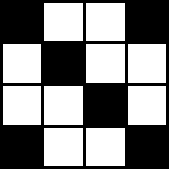
\includegraphics{images/ausfuell-1.pdf}
\qquad
\qquad
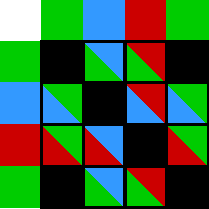
\includegraphics{images/ausfuell-2.pdf}
\caption{Ausfüllrätsel zum Grapheinfärbeproblem aus
Abbildung~\ref{vertex-coloring-examples}, links das leere `Spielfeld',
rechts ausgefüllt mit den Farben der Knoten.
\label{ausfuell:coloring}}
\end{figure}
Sehr viele Rätsel werden auf einem rechteckigen Feld von Zellen
bespielt, in die man etwas eintragen muss.
Sogar das Graphenfärbeproblem (\textsl{VERTEX-COLORING}) kann man
so auffassen.
Dazu formt man den gegebenen Graphen mit $n$ in eine
$n\times n$-Tabelle um, die Zeilen und Spalten entsprechen den Knoten
des Graphen, die Felder den möglichen Kanten.
Alle Felder, die zu im Graphen nicht existierenden Kanten gehören,
werden schwarz gefärbt.
In die weissen Felder müssen jetzt Paare von verschiedenen Farben
eingetragen werden, so dass in jeder Zeile die erste Farbe immer
gleich ist, und in jeder Spalte die zweite Farbe.
Ausserdem muss die Farbe einer Spalte und der entsprechenden Zeile
gleich sein.
Der Graph ist einffärbbar, wenn es möglich ist, die Tabelle wie
beschrieben auszufüllen (Abbildung~\ref{ausfuell:coloring}).

\begin{definition}
Ein {\em polynomielles Ausfüllrätsel} ist eine $n\times m$-Tabelle,
in die Zeichen eines Alphabets $\Sigma$ eingefüllt werden müssen,
so dass gewisse Regeln eingehalten werden.
Die einzuhaltenden Regeln können durch eine logische Formel beschrieben
werden, die in einer Zeit polynomiell in $nm$ berechnet werden kann.
\end{definition}

Die Bedingung der Berechenbarkeit in polynomieller Zeit ist meistens
offensichtlich.
Oft entsteht die Formel nämlich durch Anpassung der immer gleichen
Regeln für jedes Feld.
In solchen Fällen genügt es, wenn die resultierende Formel polynomielle
Länge hat.

\begin{beispiel}
Die Formel, die die Sudoku-Regeln für das $n^2\times n^2$-beschreibt,
besteht aus einer 
Teilformel für jedes Feld, welche wiederum aus einer Teilformel
für Zeilen, Spalten und Unterfelder besteht.
Diese Teilformeln überprüfen die Werte aller $n^2$ Felder der Zeile,
Spalte oder des Unterfeldes, dabei sind $n^2$ mögliche Feldinhalte
zu berücksichtigen.
Im Abschnitt~\ref{subsection:sudoku-und-sat} wurde gezeigt, wie die
Teilformel aufzubauen ist, ihre Länge ist
\[
O(\underbrace{n^2}_{\text{Vergleichsfelder}}\cdot
\underbrace{n^2}_{\text{Zeichen}}) = O(n^4).
\]
Die gesamte Formel hat damit die Länge
\[
O(\underbrace{n^4}_{\text{Felder}}\cdot
\underbrace{n^2}_{\text{Vergleichsfelder}}\cdot
\underbrace{n^2}_{\text{Zeichen}}) = O(n^8).
\]
Insbesondere ist die Länge der Formel polynomiell in der Feldgrösse $n^4$,
\textsl{SUDOKU}
ist also ein polynomielles Ausfüllrätsel im genannten Sinn.
\end{beispiel}

\begin{satz}
Ein polynomielles Ausfüllrätsel $A$ lässt sich polynomiell auf 
\textsl{SAT} reduzieren.
\end{satz}

\begin{proof}[Beweis]
Polynomielle Reduktion auf \textsl{SAT} bedeutet, dass man zu jeder
Probleminstanz eine logische Formel $\varphi$ konstruieren muss,
deren Länge polynomiell in der Grösse des Ausgangsproblems ist.
Die Formel muss genau dann erfüllbar sein, wenn das ursprüngliche
Problem lösbar ist.
Ein polynomielles Ausfüllrätsel führt aber nach Definition auf
eine solche Formel.
\end{proof}

Als Konsequenz dieser Konstruktion können wir auch schliessen, dass
jedes Ausfüllrätsel in NP liegt.



\subsection{Beweis des Satzes von Cook-Levin}

NP-vollständig heisst, dass jedes beliebige Problem in polynomieller
Zeit auf ein \textsl{SAT}-Problem reduziert werden kann.
Wir müssen
also einen Algorithmus angeben, mit dem aus einer Turingmachine
$M$ und einem Wort $w$
eine logische Formel $\varphi$ konstruiert werden kann, die genau
dann erfüllbar ist, wenn die Turingmaschine $M$ das Wort $w$
akzeptieren kann.

Die nicht deterministische Turingmaschine $M$ hat polynomielle Laufzeit,
jede Berechnung auf Inputwörter der Länge $n$ ist einer Zeit $n^k$
abgeschlossen. In dieser Zeit kann die Maschine höchstens $n^k$ Felder
des Bandes beschreiben, es wird also höchstens ein Abschnitt der
Länge $n^k$ des Bandes benutzt. Dabei werden maximal $n^k$
Konfigurationen durchlaufen. Schreibt man diese untereinander,
haben alle Konfigurationen in einem Quadrat $n^k\times n^k$
Platz.

Die Aufgabe ist jetzt also, das $n^k \times n^k$-Quadrat so mit Zuständen
und Symbolen auszufüllen, dass eine gültige Berechnung beschrieben wird,
die im Zustand $q_{\text{accept}}$ endet.
Dies ist ein Ausfüll-Rätsel, es bleibt uns also nur noch zu verstehen,
dass es sich auch um ein polynomielles Ausfüllrätsel handelt,
dass wir also die Bedingungen, denen die Symbole unterworfen sind,
in eine polynomielle Formel gefasst werden können.

Wir möchten jetzt also eine Formel aufstellen, die genau dann wahr
ist, wenn sich in das Quadrat $n^k\times n^k$ die Bandsymbole und
Zustände so hineinschreiben lassen, dass die Konfigurationen eine
Abfolge beschreiben, die einer gültigen Berechnung entsprechen.

Die einzelnen Zellen $c_{ij}$ der Tabelle sind mit einer Zeilennummer $i$
und einer Spaltennummer $j$ indiziert, in jede Zelle kann
genau ein Zeichen $z_{ij}$ geschrieben werden.
Zeichen können entweder Bandalphabetzeichen oder Zustände sein.
Der grösseren Einheitlichkeit wegen markieren wir die Enden des verwendeten
Bandabschnittes mit einem weiteren, bisher unbenutzten Zeichen {\tt\#}.
In einer Zelle finden wir also immer ein Zeichen aus $C=Q\cup \Gamma\cup\{\text{\tt\#}\}$.
Wir verwenden die logischen
Variablen $x_{ijs}$ mit $1\le i,j\le n^k$ und $s\in C$, die
genau dann wahr ist, wenn die Zelle $c_{ij}$ das Zeichen $s$ enthält.

Wir wissen bereits aus Satz~\ref{skript:satz:vergleichsformel}, dass wir
eine Vergleichsformel polynomiell in eine logische Formel umwandeln
können, es ist also nur noch nötig, die Bedingungen für das Ausfüllrätsel
als Vergleichsformel zu schrieben.

%In jede Zelle muss genau ein Zeichen geschrieben werden. Damit die Zelle
%$c_{ij}$ ein Zeichen enthält, muss mindestens eine der Variablen $x_{ijs}$
%wahr sein. Es dürfen aber keine zwei Zeichen einer Zelle zugeordnet sein,
%$x_{ijs}\wedge x_{ijt}$ für zwei verschiedenen Zeichen $s$ und $t$ darf
%also nicht wahr sein. Also muss jede Formel
%$\neg(x_{ijs}\wedge x_{ijt})=\overline{x_{ijs}}\vee\overline{x_{ijt}}$
%für zwei verschiedene Zeichen wahr sein, zusammen mit der
%Bedingung, dass ein Zeichen in der Zelle steht, erhalten wir
%für die Zellen $c_{ij}$ die Formel
%\[
%\varphi_{c_{ij}}=
%\biggl(\bigvee_{s\in C} x_{ijs}\biggr)\wedge
%\bigwedge_{\myatop{s,t\in C}{s\ne t}} (\overline{x_{ijs}}\vee\overline{x_{ijt}}).
%\]
%Dies muss für jede Indexkombination gelten, also
%\[
%\varphi_c
%=
%\bigwedge_{1\le i,j\le n^k}
%\varphi_{c_{ij}}
%=
%\bigwedge_{1\le i,j\le n^k}\biggl(
%\biggl(\bigvee_{s\in C} x_{ijs}\biggr)\wedge
%\bigwedge_{\myatop{s,t\in C}{s\ne t}} (\overline{x_{ijs}}\vee\overline{x_{ijt}})
%\biggr).
%\]
%Da unsere Redukton polynomiell sein soll, müssen wir auch bestimmen,
%wie lang die Formel $\varphi_c$ ist. Alle Formeln $\varphi_{c_{ij}}$
%sind gleich gross, abhängig nur von $|C|$, also einer Konstanten.
%Damit ist die Länge von $\varphi_c$ bestimmt durch die Grösse der
%Tabelle, also $O(n^2k)$. Die zum Aufbau von $\varphi_c$ notwendig Zeit
%ist ebenfalls $O(n^2k)$.

\subsubsection{Start mit dem Wort $w$}
Als nächstes drücken wir in einer Formel $\varphi_i$ aus,
dass die Turingmaschine mit dem
Wort $w$ initialisiert worden ist. Dazu muss in irgendeiner
Zelle der ersten Zeile das Zeichen $q_0$ stehen, und rechts
anschliessen die Zeichen des Wortes $w=a_1a_2\dots a_{|w|}$.
Steht $q_0$ in der
Zelle $j$, wird die Formel
\[
\varphi_{\text{start},j}
=
x_{11\#}\wedge
x_{12\blank}\wedge \dots \wedge
x_{1,j-1,\blank}\wedge
x_{1,j,q_0}\wedge
x_{1,j+1,a_1}\wedge\dots\wedge
x_{1,j+|w|,a_{|w|}}\wedge
x_{1,j+|w|+1,\blank}\wedge\dots\wedge
x_{1,n^k,\#}
\]
wahr.
Soll der Initialisierungsstring irgendwo in der ersten Zeile
stehen, wird eine der Formeln war, also
\[
\varphi_{\text{start}} = \bigvee_{1\le j\le n^k} \varphi_{\text{start}_j}.
\]
Auch diese Formel ist nicht grösser als $O(n^{2k})$ und kann in
polynomieller Zeit erzeugt werden.

\subsubsection{Akzeptierzustand}
In der letzten Zeile der Tabelle muss der Zustand $q_\text{accept}$ stehen,
wir können dies durch den 
Irgendwo in der Tabelle muss der Akzeptierzustand stehen, also
\[
\varphi_{\text{accept}} 
=
\bigvee_{1\le i\le n^k} x_{N,i,q_{\text{accept}}}.
\]
ausdrücken.

\subsubsection{Berechnungsgeschichte}
Die Konfigurationen in der Tabelle müssen alle durch
Turingmaschinenübergänge auseinander hervorgehen, die Tabelle muss
mit einer Berechnungsgeschichte ausgefüllt werden.
Ob dies der Fall ist, kann durch die Betrachtung von zwei Zeilen
hohen und drei Zellen breiten Ausschnitten aus der Tabelle
überprüft werden.
Solche Ausschnitte zeigen fast immer zwei
gleiche Zeilen, ausser an der aktuellen Kopfposition, wo
sich etwas ändern kann.

Ein Übergang
\[
\entrymodifiers={++[o][F]}
\xymatrix{
p\ar[r]^{a\to b,R}
	&q
}
\]
wird zum Beispiel in den Ausschnitten
\[
\begin{tabular}{|c|c|c|}
\hline
$x$&$y$&$p$\\
\hline
$x$&$y$&$b$\\
\hline
\end{tabular}
\quad
\begin{tabular}{|c|c|c|}
\hline
$y$&$p$&$a$\\
\hline
$y$&$b$&$q$\\
\hline
\end{tabular}
\quad
\begin{tabular}{|c|c|c|}
\hline
$p$&$a$&$x$\\
\hline
$b$&$q$&$x$\\
\hline
\end{tabular}
\quad
\begin{tabular}{|c|c|c|}
\hline
$a$&$x$&$y$\\
\hline
$q$&$x$&$y$\\
\hline
\end{tabular}
\]
sichtbar. Ein Übergang mit einer Kopfbewegung nach links
\[
\entrymodifiers={++[o][F]}
\xymatrix{
p\ar[r]^{a\to b,L}
	&q
}
\]
dagegen in den Ausschnitten
\[
\begin{tabular}{|c|c|c|}
\hline
$z$&$x$&$y$\\
\hline
$z$&$x$&$q$\\
\hline
\end{tabular}
\quad
\begin{tabular}{|c|c|c|}
\hline
$x$&$y$&$p$\\
\hline
$x$&$q$&$y$\\
\hline
\end{tabular}
\quad
\begin{tabular}{|c|c|c|}
\hline
$y$&$p$&$a$\\
\hline
$q$&$y$&$b$\\
\hline
\end{tabular}
\quad
\begin{tabular}{|c|c|c|}
\hline
$p$&$a$&$x$\\
\hline
$y$&$b$&$x$\\
\hline
\end{tabular}
\quad
\begin{tabular}{|c|c|c|}
\hline
$a$&$x$&$y$\\
\hline
$b$&$x$&$y$\\
\hline
\end{tabular}
\]
Es gibt eine endliche Anzahl korrekter Belegungen solcher
$2\times 3$-Ausschnitte mit den Zeichen aus $C$, die Anzahl
hängt nur von $|C|$ und den Übergängen der Turingmaschine ab.

Jetzt müssen wir zeigen, dass wir gültige Übergänge, die durch erlaubte
Inhalte von $2\times 3$-Ausschnitten charakterisiert sind, mit
einer Vergleichsformel erkennen können.
Wir können aber für jede Ausschnitt-Position eine Vergleichsformel
aufstellen, die wahr wird, wenn die Zeichen im Ausschnitt 
gleich sind zu einem erlaubten Ausschnitt.
Insbesondere gibt es eine Vergleichsformel für Ausschnitt-Inhalte.

%Die Belegung
%\[
%\begin{tabular}{|c|c|c|}
%\hline
%$a_1$&$a_2$&$a_3$\\
%\hline
%$a_4$&$a_5$&$a_6$\\
%\hline
%\end{tabular}
%\]
%eines Ausschnitts mit der Zelle $c_{ij}$ in der
%linken oberen Ecke entspricht 
%\[
%x_{i,j,a_1}\wedge
%x_{i+1,j,a_2}\wedge
%x_{i+2,j,a_3}\wedge
%x_{i,j+1,a_4}\wedge
%x_{i+1,j+1,a_5}\wedge
%x_{i+2,j+1,a_6}.
%\]
%Davon muss eine wahr sein, also
%\[
%\varphi_{\text{Ausschnitt}_{ij}}
%=
%\bigvee_{\text{$a_1,\dots,a_6$ korrekt}}
%x_{i,j,a_1}\wedge
%x_{i+1,j,a_2}\wedge
%x_{i+2,j,a_3}\wedge
%x_{i,j+1,a_4}\wedge
%x_{i+1,j+1,a_5}\wedge
%x_{i+2,j+1,a_6}.
%\]
%Ausserdem muss jeder Ausschnitt gültig belegt sein, also
%muss
%\[
%\varphi_{\text{Ausschnitt}} =\bigwedge_{1\le i,j\le n^k}\varphi_{\text{Ausschnitt}_{ij}}
%\]
%wahr sein. Auch diese Formel lässt sich in polynomieller Zeit konstruieren
%und sie hat polynomielle Länge.

\subsubsection{Maschine hält auf einem Akzeptierzustand an}
Die Maschine kann schon wesentlich früher anhalten, also die worst case
Laufzeit anzeigt.
Wir müssen die Tabelle daher nach Ende der Berechnung mit immer gleichen
Zeilen ausfüllen.
Wir können dies erreichen, indem wir den erlaubten Ausschnitt-Inhalten
die drei Ausschnitte
\[
\begin{tabular}{|>{$}c<{$}|>{$}c<{$}|>{$}c<{$}|}
\hline
q_*&x&y\\
\hline
q_*&x&y\\
\hline
\end{tabular}
\qquad\text{oder}\qquad
\begin{tabular}{|>{$}c<{$}|>{$}c<{$}|>{$}c<{$}|}
\hline
x&q_*&y\\
\hline
x&q_*&y\\
\hline
\end{tabular}
\qquad\text{oder}\qquad
\begin{tabular}{|>{$}c<{$}|>{$}c<{$}|>{$}c<{$}|}
\hline
x&y&q_*\\
\hline
x&y&q_*\\
\hline
\end{tabular}
\]
mit $q_*\in\{q_\text{accept},q_\text{reject}\}$ und beliebigen
Bandalphabetzeichen $x$ und $y$ hinzufügen.

Wir haben also mehrere logische Formeln und Vergleichsformeln
gefunden, die genau dann alle wahr sind, wenn die Tabelle mit einer
akzeptierenden Berechnungsgeschichte gefüllt ist.
Die einzelnen Teile sind von polynomieller Grösse, also auch deren
Konjunktion.
Damit ist gezeigt, dass sich $A$ polynomiell auf ein polynomielles
Ausfüllrätsel reduzieren lässt.

%Damit die Tabelle eine akzeptierende Berechnung beschreibt, müssen
%alle Teile wahr sein, also ist
%\[
%\varphi =
%\varphi_{c}\wedge
%\varphi_{\text{start}}\wedge
%\varphi_{\text{accept}}\wedge
%\varphi_{\text{Ausschnitt}}
%\]
%die gesuchte Formel, die genau dann erfüllbar ist, wenn $w$ von der
%Turingmaschine $M$ akzeptiert werden kann.

